\section{Модель термической деполимеризации ПММА} \label{sec:depolymerization}

В данном разделе описывается подход, который был разработан для моделирования распределения среднечисловой молекулярной массы \linebreak ПММА в различные моменты процесса СЭЛТР.
Начальные значения среднечисловой ($\Mn$) и средневесовой ($\Mw$) молекулярной массы ПММА были приняты равными 271000 и 669000 соответственно, что соответствует резисту PMMA 950K A2 от компании <<Allresist>>, использовавшемуся в данной работе.
Предполагалось, что экспонирование производится ``в~кадр'' (вдоль серии параллельных линий), величина тока экспонирования была принята равной 5~нА, энергия электронного пучка -- 20 кэВ, размеры экспонируемой области -- \linebreak 2.4$\times$1.9 мм$\pp$, толщина слоя ПММА -- 500 нм, расстояние между линиями -- 3 мкм, время экспонирования -- 100 с, температура образца -- 130~$^\circ$C.
Данные значения согласуются со значениями соответствующих параметров в ранее проводившихся экспериментах по изучению метода СЭЛТР~\cite{Bruk_2016_mee}.
Число линий, получаемых при экспонировании ``в кадр'' составляет 625, однако для уменьшения требуемого машинного времени моделирование проводилось для участка одной линии длиной 100~нм с использованием периодических граничных условий.
На основе промоделированного распределения актов электрон-электронного взаимодействия в слое ПММА и вероятности разрыва (0.083 для 130~$^\circ$C) рассчитывалось распределение числа разрывов молекул ПММА.
$x-$ и $z-$координаты актов разрыва записывались в двумерную гистограмму с размером бина 50 нм по обеим осям.
Примеры гистограмм, отображающих распределение концентрации разрывов молекул ПММА при различных значений времени экспонирования, приведены на рисунке~\ref{fig:scission_hist}.

\begin{figure}[t]
	\begin{center}
		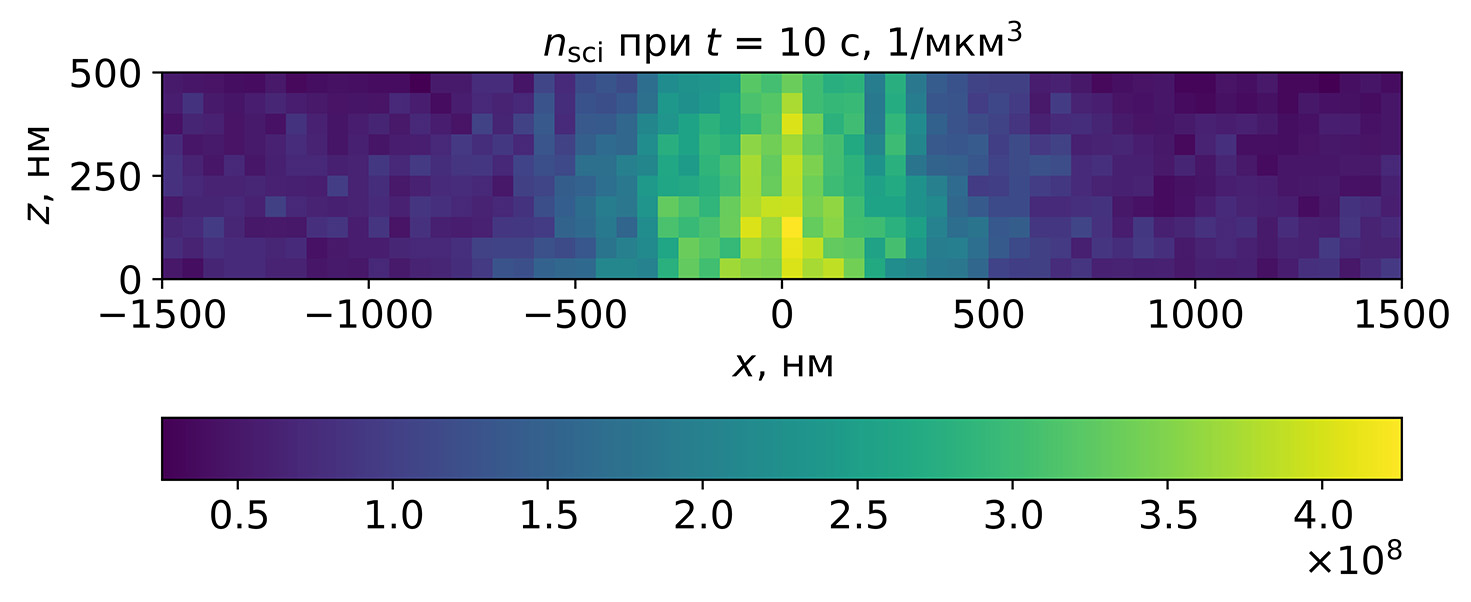
\includegraphics[width=0.8\linewidth]{MW/sci_conc_10s_straight_200} \\
		\vspace{-3.7em} \text{\hspace{-26em} a)} \vspace{2.7em} \\
		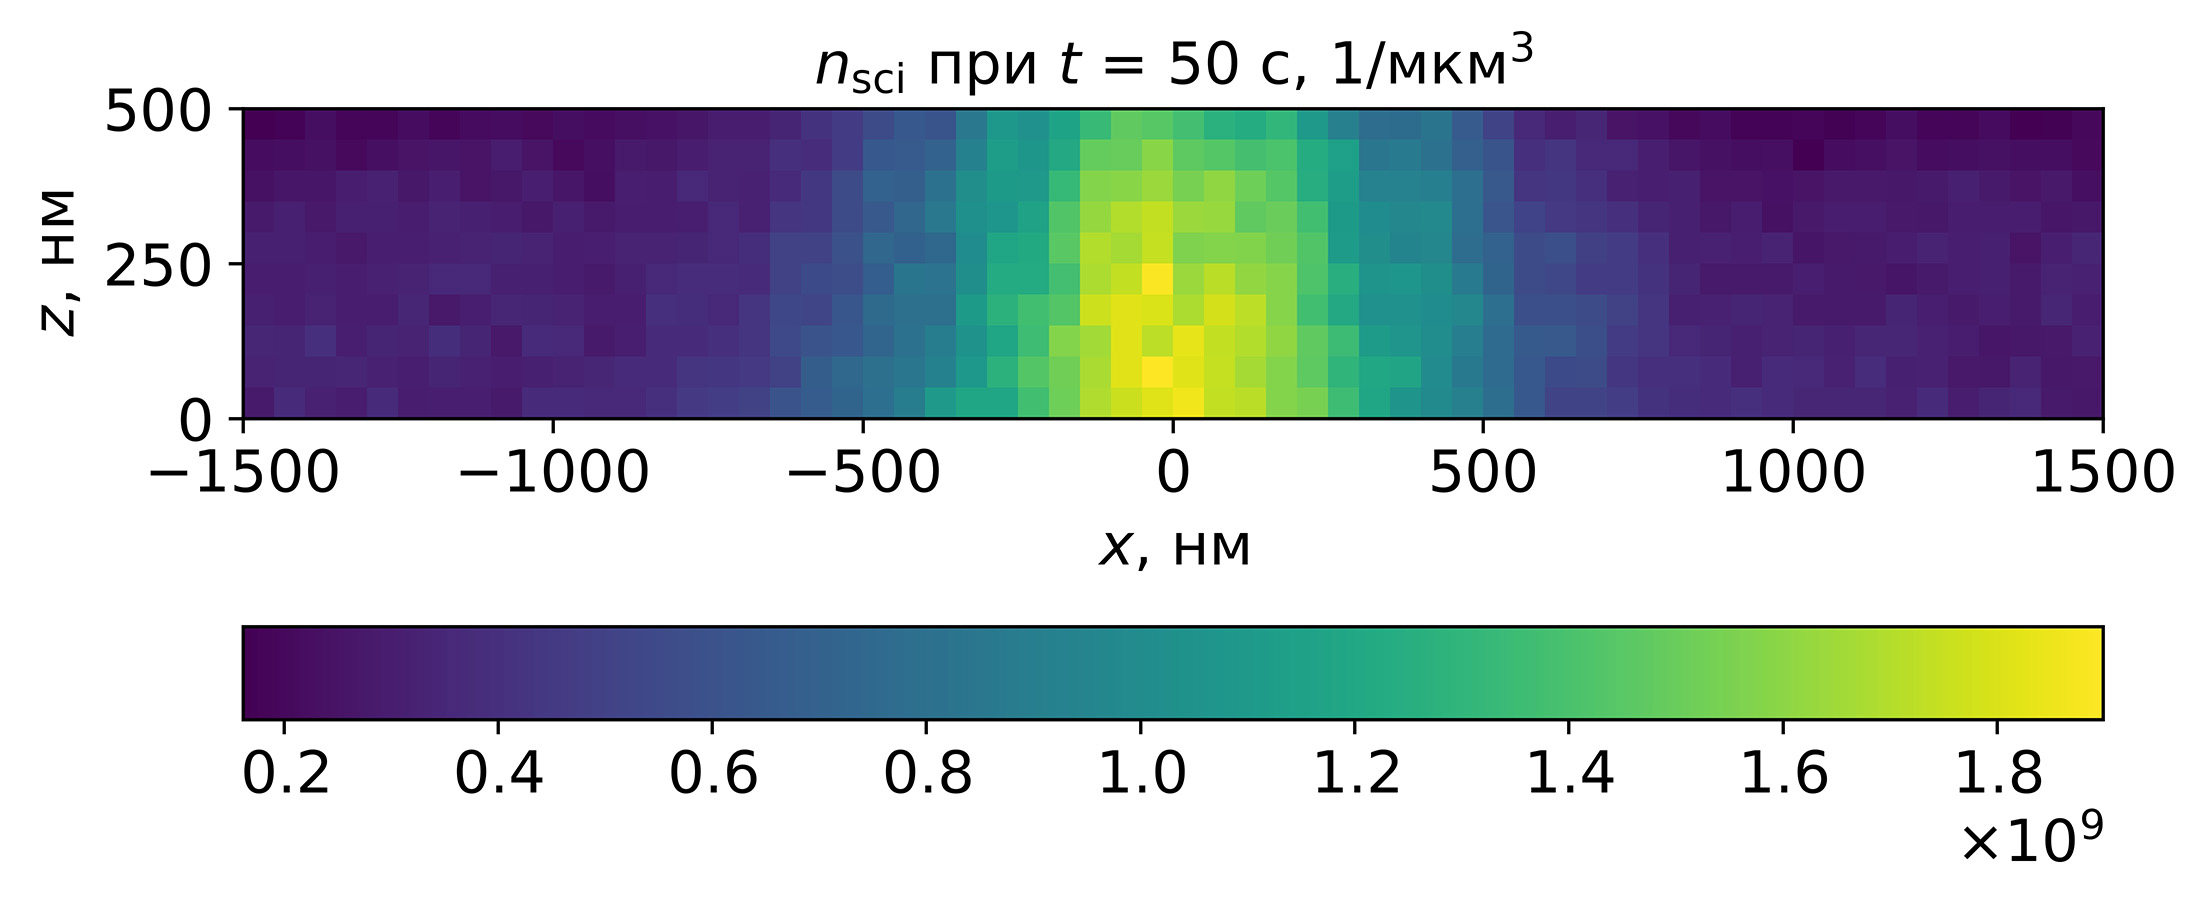
\includegraphics[width=0.8\linewidth]{MW/sci_conc_50s_straight_200} \\
		\vspace{-3.7em} \text{\hspace{-26em} б)} \vspace{3.7em} \\
	\end{center}
	\vspace{-2.5em}
	\caption{
		Промоделированные распределения концентрации разрывов молекул в слое ПММА при температуре 130~$^\circ$C.
		Экспонирование производилось ``в~кадр'', размеры кадра составляли 2.4$\times$1.9 мм$\pp$, число линий в кадре -- 625, расстояние между линиями -- 3 мкм, время экспонирования составляло 10 с (а) и 50 с (б).
		Энергия электронного пучка равна 20 кэВ, ток экспонирования -- 5~нА. Моделирование проводилось в пределах одной линии с периодическими граничными условиями.}
	\label{fig:scission_hist}
\end{figure}

Для моделирования молекулярно-массового распределения ПММА была использована модель, описанная в разделе~\ref{sec:depolymerization}.
Использовалось предположение о том, что молекулярно-массовое распределение ПММА описывается функцией распределения Шульца-Цимма со значениями среднечисловой и средневесовой молекулярной массы, равными 271000 и 669000 соответственно:
\begin{equation} \label{eq:Schulz-Zimm_distribution}
	P_n = C_0 n^z \exp (-n/y).
\end{equation}
Начальные значения параметров этого распределения ($z_0$ и $y_0$) были найдены на основе формул \ref{eq:Schulz-Zimm_1} и \ref{eq:Schulz-Zimm_2}:
\begin{equation}
	\begin{aligned}
		PD & \equiv \frac{\Mw}{\Mn} = \frac{669000}{271000} \cong 2.47, \\
		z_0 & = (2-PD)/(PD-1) \cong -0.32, \\
		y_0 & = x_0/(z_0+1) \cong 3989.58.
	\end{aligned}
\end{equation}
Также, согласно результатам работы~\cite{Mita_PMMA_zip_lengths_T}, средняя длина цепи деполимеризации при 130~$^\circ$C была принята равной 500.
После задания всех параметров система дифференциальных уравнений~\ref{eq:scary_system} решалась численно методом Рунге-Кутты 4 порядка с переходом на схему предиктор-корректор начиная с четвертого шага (рисунок~\ref{fig:SZ_M1_y_tau}).
Диапазон значений переменной $\tau$ составлял от 0 до 400 с шагом 0.01.
\begin{figure}[t]
	\begin{minipage}{0.48\textwidth}
			\hspace{-0.5em} 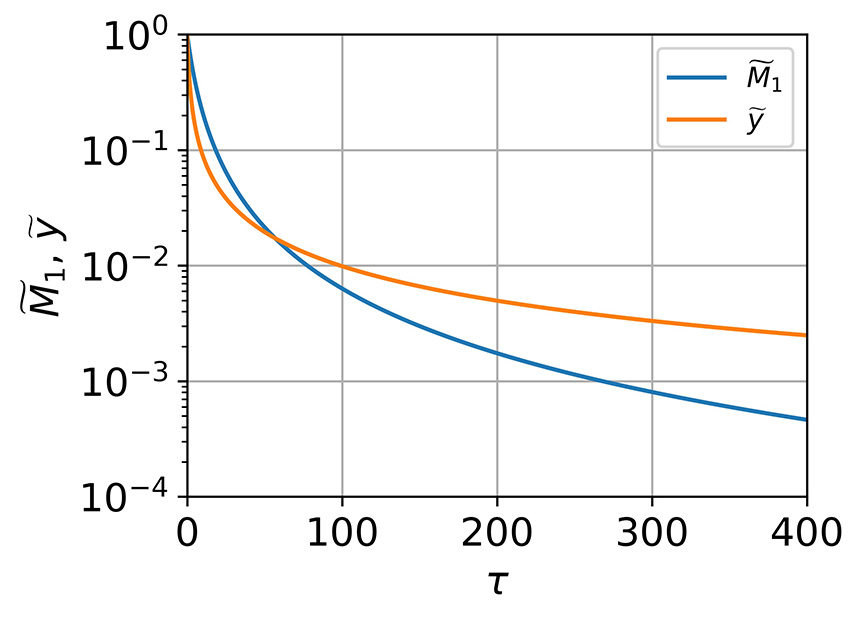
\includegraphics[width=\linewidth]{MW/SZ_M1_y_14_200} \\
			\vspace{-12.5ex} \\ \text{\hspace{3.8em} a}) \\ \vspace{12.5ex}
		\end{minipage}
	\begin{minipage}{0.48\textwidth}
			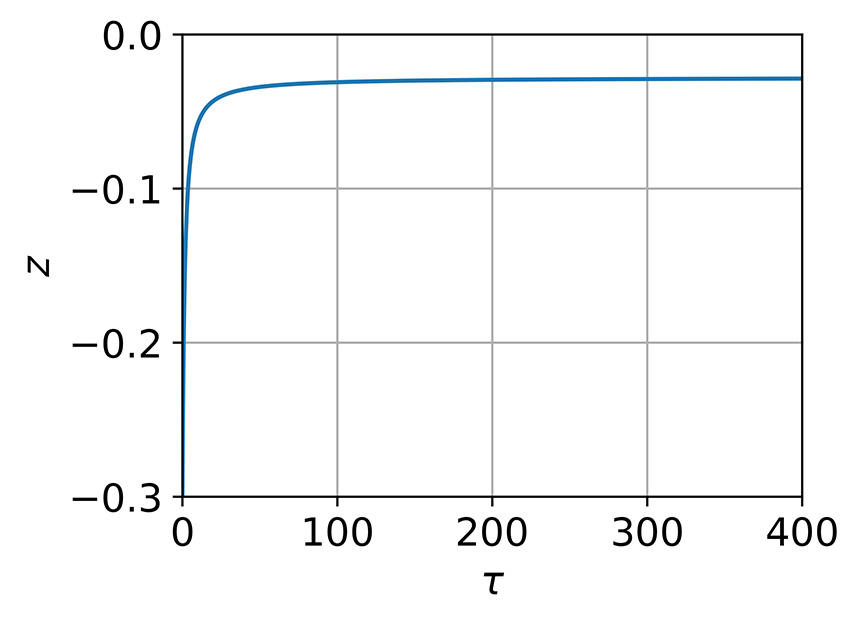
\includegraphics[width=\linewidth]{MW/SZ_z_14_200} \\
			\vspace{-12.5ex} \\ \text{\hspace{4em} б}) \\ \vspace{12.5ex}
		\end{minipage}
	\vspace{-3.5em}
	\caption{
		Зависимости параметров распределения Шульца-Цимма $\tilde{M_1}$, $\tilde{y}$ (а) и $z$ (б) от безразмерной временной переменной $\tau$, полученные для резиста PMMA 950K A2, использовавшегося в данной работе.
	}
	\label{fig:SZ_M1_y_tau}
\end{figure}
Зависимости параметров распределения молекулярной массы резиста от безразмерной переменной $\tau$ далее пересчитывались в зависимости от времени экспонирования $t$ по формуле~\ref{eq:dim_less_MW}:
\begin{equation} \label{eq:tau_y0_ks_t}
	\tau = y_0 k_\mathrm{s} t.
\end{equation}

Входящая в это выражение величина $k_\mathrm{s}$, выражающая число активных центров деполимеризации, появляющихся за 1 с, приходящееся на один мономер, определялась следующим образом.
Изначально была создана двумерная гистограмма с размерами, аналогичными размерам гистограммы для распределения числа разрывов, в каждую ячейку которой (условно с индексами $i$ и $j$) в качестве начального значения величины $\tau$ было записано число 0.
Далее для каждой секунды экспонирования моделировалось число разрывов молекул ПММА, относившихся к этой ячейке ($N_\mathrm{sci}^\mathrm{1c}[i,j]$).
При этом считалось, что число активных центров деполимеризации, появлявшихся за 1 с в данной ячейке, равнялось числу промоделированных разрывов полимерных молекул в ячейке.
После этого прибавка к величине $\tau$ в данной ячейке, соответствующая 1 секунде экспонирования, определялась по формуле~\ref{eq:tau_y0_ks_t}:
\begin{equation}
	\Delta \tau_\mathrm{1c} [i,j] = 3989.58 \cdot \frac{N_\mathrm{sci}^\mathrm{1c}[i,j]}{1789618} \cdot 1с,
\end{equation}
где 1789618 -- число мономеров в одной ячейке гистограммы (область размерами 50$\times$100$\times$50 нм$\ppp$), рассчитанное на основе плотности ПММА и молярной массы ММА (1.19~г/см$\ppp$ и 100 г/моль соответственно).
Величина $\Delta \tau_\mathrm{1c} [i,j]$ добавлялась к текущему значению $\tau$ для данной ячейки и далее для нового значения $\tau$ определялись соответствующие значения параметров $y$ и $z$ молекулярно-массового распределения ПММА.
Такой подход позволял вычислить локальные значения среднечисловой массы ПММА в различные моменты времени экспонирования по формуле
\begin{equation}
	M_\mathrm{n} [i,j] (t) = y[i,j] (t) (z [i,j] (t) + 1).
\end{equation}
Промоделированные таким образом пространственные распределения локальной среднечисловой молекулярной массы ПММА для двух различных значений времени экспонирования приведены на рисунке~\ref{fig:Mn_hist}.

\begin{figure}[h]
	\begin{center}
		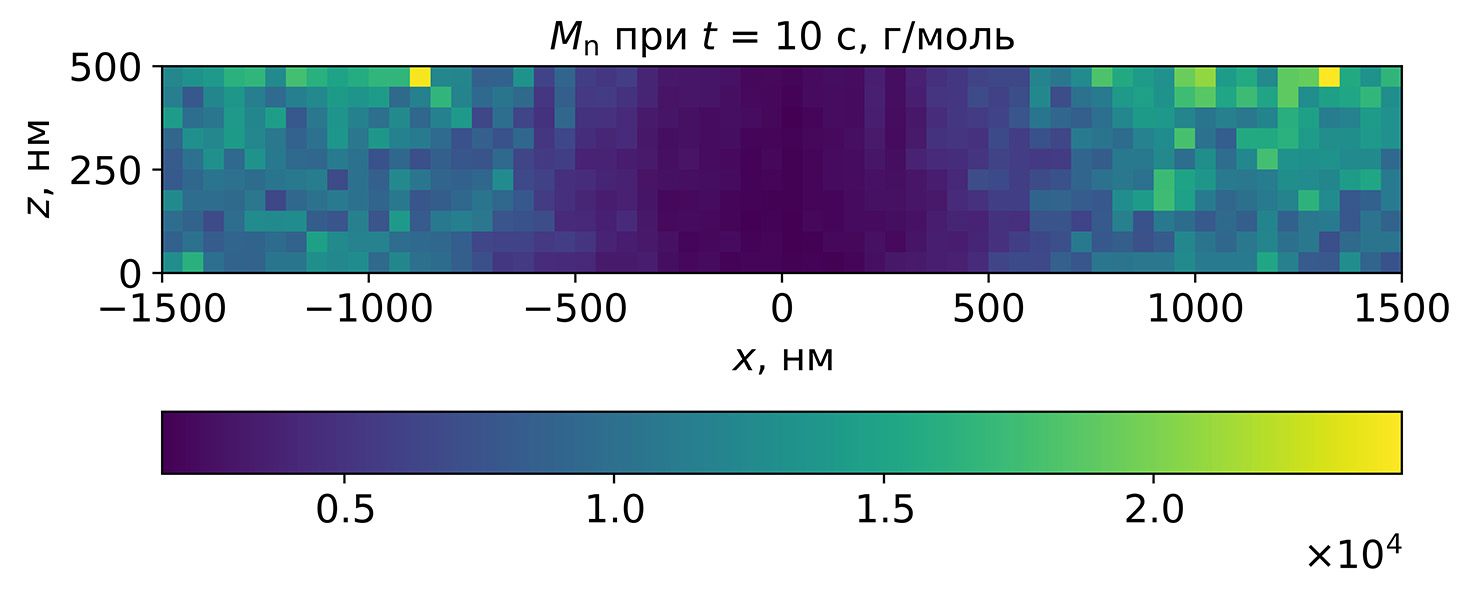
\includegraphics[width=0.8\linewidth]{MW/Mn_hist_10s_straight_200} \\
		\vspace{-3.7em} \text{\hspace{-26em} a)} \vspace{2.7em} \\
		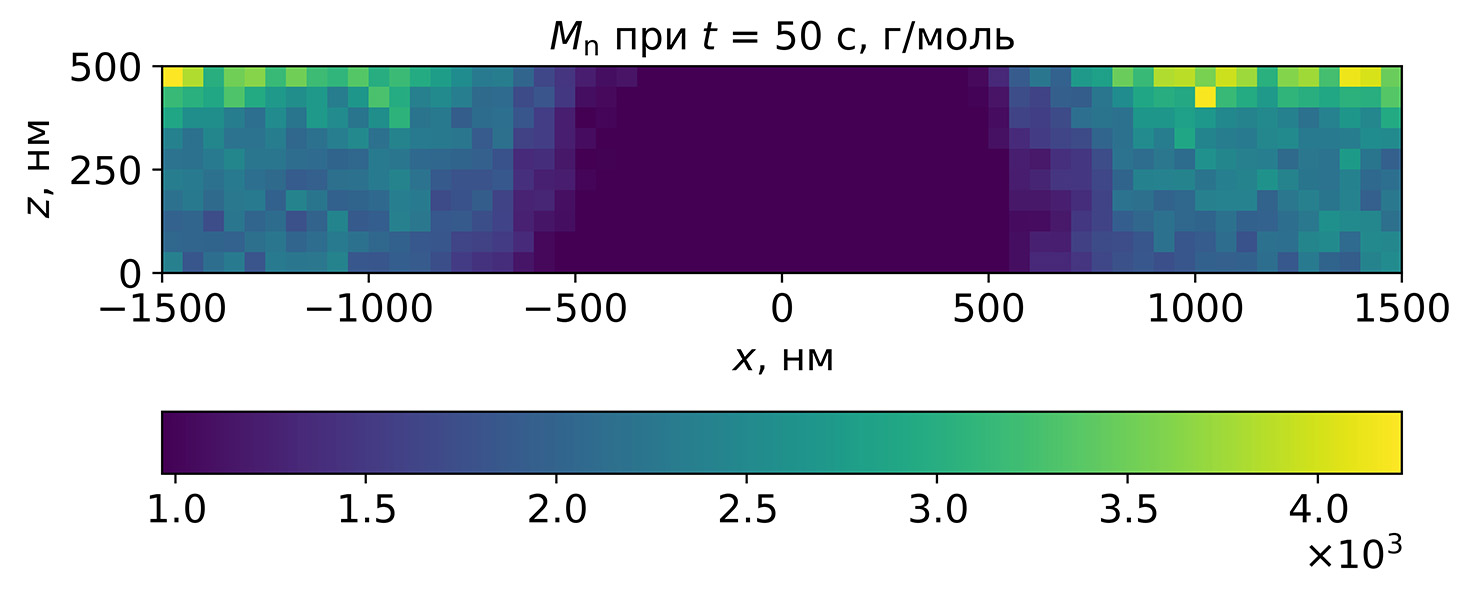
\includegraphics[width=0.8\linewidth]{MW/Mn_hist_50s_straight_200} \\
		\vspace{-3.7em} \text{\hspace{-26em} б)} \vspace{3.7em} \\
	\end{center}
	\vspace{-2.5em}
	\caption{
		Промоделированные распределения локальной среднечисловой молекулярной массы PMMA 950К A2 при температуре 130~$^\circ$C.
		Экспонирование производилось ``в~кадр'', размеры кадра составляли 2.4$\times$1.9 мм$\pp$, число линий в кадре -- 625, расстояние между линиями -- 3 мкм, время экспонирования составляло 10 с (а) и 50 с (б).
		Энергия электронного пучка равна 20 кэВ, ток экспонирования -- 5~нА. Моделирование проводилось в пределах одной линии с периодическими граничными условиями.}
	\label{fig:Mn_hist}
\end{figure}
